\section{GKP codes}\label{sec:gkp-codes}

As mentioned at the start of this chapter, GKP codes~\cite{Gottesman_2001} can be viewed as the generalisation to the CV case of Pauli qubit stabilizer codes.
Unlike in \Cref{ch:qubit_prelims}, where we went into a fair amount of detail about stabilizer codes, here we write the minimum needed to fully define GKP codes, then look at some examples.
All content in this section is taken from a combination of \Ccite{Conrad2024thesis,Burchards_2025}
We start by defining \textit{lattices}.

\subsection{Lattices}

We will define a (real) \textit{lattice} to be a \textit{discrete} subgroup $\Lambda$ of a (real) vector space $\VVV$, where discrete means every point $\bsym{\eta} \in \Lambda$ has some open ball around it containing no other lattice points.
(A real vector space is a metric space, so `open balls' are well-defined.)
We define the rank of a lattice to be the dimension of the vector space spanned by its points.
A lattice is then full-rank iff $\rank(\Lambda) = \rank(\VVV)$.
If $\VVV$ is in fact a \textit{symplectic} vector space with symplectic product $\odot$, we can go further.
As a reminder, we can always view $\VVV = \mathbb{R}^{2n}$ as a symplectic vector space via the standard symplectic product $\binom{\bsym{v}}{\bsym{u}} \odot \binom{\bsym{v}'}{\bsym{u}'} = \bsym{v} \cdot \bsym{u'} - \bsym{u} \cdot \bsym{v'}$.
For such $V$, we can define the (symplectic) dual lattice:
\begin{equation}\label{eq:sympletic_dual_lattice}
    \Lambda^{\perp} \coloneqq \{\bsym{\eta} \in \VVV \mid \forall \bsym{\xi} \in \Lambda,\ \bsym{\eta} \odot \bsym{\xi} \in \mathbb{Z}\}
\end{equation}
A lattice $\Lambda$ is then (symplectically) integral iff $\Lambda \leq \Lambda^\perp$, and (symplectically) self-dual iff in fact $\Lambda = \Lambda^\perp$.
One often sees a set of generating vectors $\bsym{\eta}_1, \ldots, \bsym{\eta}_d$ packaged up as columns of a \textit{generating matrix} $M = (\bsym{\eta}_1\ \ldots\ \bsym{\eta}_d)$.

\subsection{GKP codes}\label{subsec:gkp}

A (non-trivial) $n$-qumode GKP code is then defined by a group of the form:
\begin{equation}\label{eq:GKP_stabilizer}
    \SSS = \langle e^{i\theta_1} \hat{D}(\bsym{\eta}_1), \ldots, e^{i\theta_{2n}} \hat{D}(\bsym{\eta}_{2n}) \rangle
\end{equation}
If this group doesn't contain $-I$, we call this a (non-trivial) stabilizer group.
As a result of not containing $-I$ (and assuming the generators are all independent), the set of vectors $\Lambda_\SSS = \{\bsym{\eta} \mid \exists \theta: e^{i\theta}D(\bsym{\eta}) \in \SSS\}$ forms a full-rank, (symplectically) integral lattice in $\mathbb{R}^{2n}$.
We call the set of phases $e^{i\theta_j}$ the \textit{sector} of the code.
The codespace $\VVV_\SSS$ is the joint $+1$ eigenspace of all the stabilizer elements.
The logical operators correspond to the points of the dual lattice; $e^{i\theta}D(\boldsymbol{\eta})$ is a logical operator of the code iff $\boldsymbol{\eta} \in \Lambda^\perp$.
Indeed, letting $M$ denote the generator matrix of the lattice $\Lambda_\SSS$, the codespace dimension is given by:
\begin{equation}
    \dim(\VVV_\SSS)^2
    = |\Lambda_\SSS^{\perp} / \Lambda_\SSS|
    = |\det(M)| / |\det(M^\perp)|
    = |\det(M)|^2
\end{equation}
The algebraic distance is defined to be the length of the vector $\boldsymbol{\eta}$ corresponding to the smallest non-trivial logical operator.
Examples will be illuminating.

\begin{example}[Square lattice single-mode GKP]\label{ex:square_gkp}
    The simplest GKP code encodes a single qubit into a single qumode using a square lattice.
    We start with the self-dual lattice $\ZZ^2$ and scale this by $\sqrt{d}$ to encode a qudit; we'll choose $d = 2$.
    This lattice $\Lambda_\SSS$ is spanned by just two vectors -- written as a generator matrix this is $\sqrt{2}I_2$.
    The stabilizer group is then generated by two displacement operators:
    \begin{equation}\label{eq:square_gkp_stabilizers}
        \SSS = \pres{\hat{X}(\sqrt{2}), \hat{Z}(\sqrt{2})}
    \end{equation}
    The symplectic dual lattice $\Lambda_\SSS^\perp$ is computed using \Cref{eq:sympletic_dual_lattice}.
    We need $\tbinom{v}{u}$ such that for all $\tbinom{a\sqrt{2}}{b\sqrt{2}} \in \Lambda$, we have:
    \begin{equation}
        \tbinom{v}{u} \odot \tbinom{a\sqrt{2}}{b\sqrt{2}} = v \cdot b\sqrt{2} - u \cdot a\sqrt{2} \in \ZZ
    \end{equation}
    Crunching the numbers gives:
    \begin{equation}
        \Lambda_\SSS^\perp = \frac{1}{\sqrt{2}} \ZZ^2
    \end{equation}
    This is again a square lattice, but with exactly half the scaling of $\Lambda_\SSS$, since $1/\sqrt{2} = 1/2 \cdot \sqrt{2}$.
    We can draw this:
    \begin{equation}
        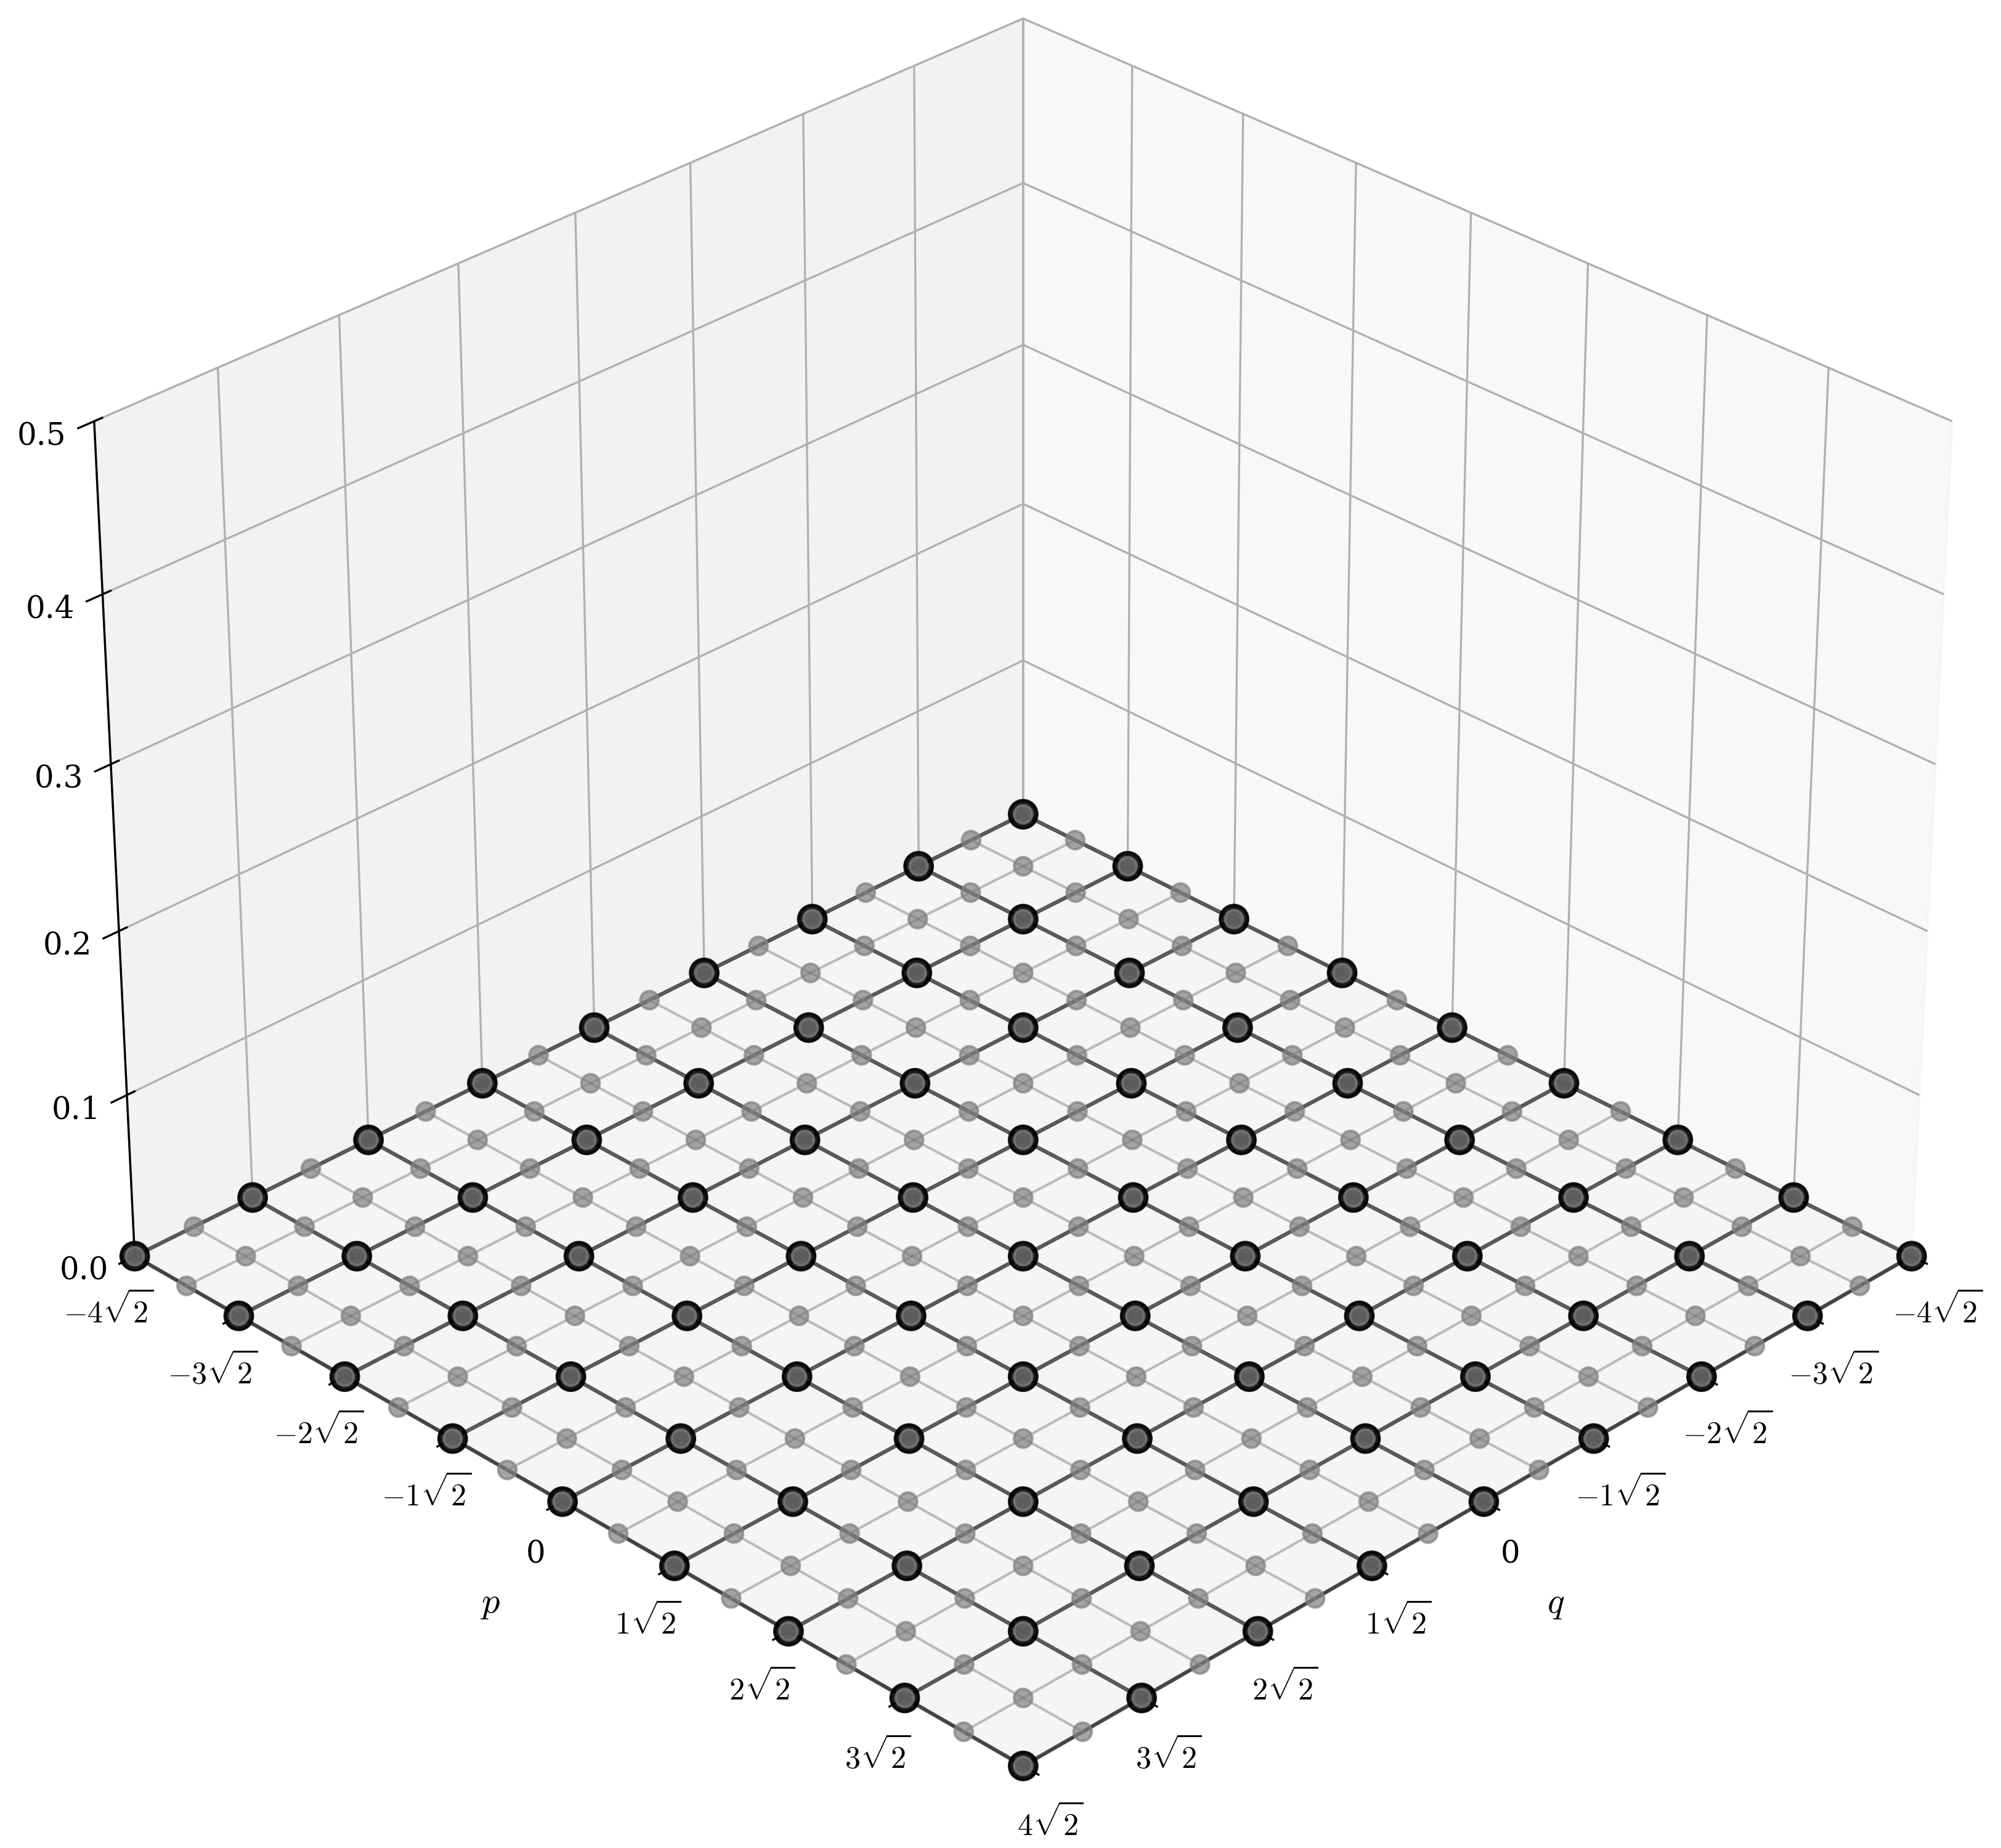
\includegraphics[valign=c, width=0.7\linewidth]{figures/qumodes/prelims/quantum_info/gkp_lattice_3d}
    \end{equation}
    Now let's determine what the codestates are.
    Any \textit{physical} state $\ket{\psi}: \mathbb{R} \to \mathbb{C}$ in the codespace must be stabilized by both generators, so we have:
    \begin{equation}
        \hat{X}(\sqrt{2})\ket{\psi} = \ket{\psi}
        \qqquad \text{and} \qqquad
        \hat{Z}(\sqrt{2})\ket{\psi} = \ket{\psi}
    \end{equation}
    Using the explicit action of displacement operators from \Cref{eq:displacement_defn_action}, the first condition gives:
    \begin{equation}
        \ket{\psi}(x - \sqrt{2}) = \ket{\psi}(x)
    \end{equation}
    So $\ket{\psi}$ must have period $\sqrt{2}$.
    The second condition gives:
    \begin{equation}
        e^{i 2\pi \sqrt{2} x} \ket{\psi}(x) = \ket{\psi}(x)
    \end{equation}
    This means that wherever $\ket{\psi}(x) \neq 0$, we must have $e^{i 2\pi \sqrt{2} x} = 1$, which requires $\sqrt{2} x \in \ZZ$.
    Therefore $\ket{\psi}$ can only have support on the discrete set of points $x \in \frac{1}{\sqrt{2}}\ZZ$.
    But here's the surprise: any such function $f$ has the property that $\int |f| = 0$, i.e.\ it's a null function.
    We said right back in \Cref{subsec:hilbert_space} that physical qumode states are elements of $\LLL^2(\RR)$, a space of equivalence classes of functions, where two functions are equivalent iff they differ by a null function.
    If $f$ is already a null function, then it's equivalent to the zero function in $\LLL^2(\RR)$.
    So the only \textit{physical} codestate is the zero function.

    Therefore, this GKP code's non-trivial codestates must be generalised codestates.
    In \Cref{subsec:qumode_evolution}, we said what it means to apply a continuous operator $U$ to a generalised state $\ket{\psi}$: we get a new generalised state $U\ket{\psi}$ that maps the Schwartz function $\ket{\phi}$ to the scalar $\ket{\psi}(U\ket{\phi})$.
    So in this case here we're looking for a functional $\ket{\psi}$ with two properties.
    Firstly, we need $\hat{X}(\sqrt{2})\ket{\psi} = \ket{\psi}$, i.e.\ for all $\ket{\phi}(x) \in \Phi$ we need:
    \begin{equation}
        \ket{\psi}(\hat{X}(\sqrt{2}) \ket{\phi}(x)) = \ket{\psi}(\ket{\phi}(x - \sqrt{2})) = \ket{\psi}(\ket{\phi}(x))
    \end{equation}
    Secondly, we need $\hat{Z}(\sqrt{2})\ket{\psi} = \ket{\psi}$, i.e.\ for all $\ket{\phi}(x) \in \Phi$ we need:
    \begin{equation}
        \ket{\psi}(\hat{Z}(\sqrt{2}) \ket{\phi}(x)) = \ket{\psi}(e^{i2\pi\sqrt{2}x}\ket{\phi}(x)) = \ket{\psi}(\ket{\phi}(x))
    \end{equation}
    It can be shown that the only functionals satisfying these condition are \textit{Dirac combs} -- periodic sums of delta distributions.
    Specifically, $\ket{\psi}$ is a codestate iff it's of the form:
    \begin{equation}\label{eq:square_gkp_dirac_comb}
        \ket{\psi} = \sum_{k \in \ZZ} c_k \delta_{k/\sqrt{2}}
    \end{equation}
    where the coefficients $c_k$ satisfy $c_{k + 2} = c_k$ due to the periodicity condition (since there are $\sqrt{2}/(1/\sqrt{2}) = 2$ `teeth' per period).
    The name comes from the informal association of the Dirac distribution $\delta_a$ with the limit of the Gaussian curve centred at $a$ as it gets narrower and taller, as in \Cref{eq:dirac_distribution_as_real_function}.
    Let's plot this -- as well as approximating each distribution by a Gaussian, we multiply the overall function by another Gaussian envelope to normalise it.
    \begin{equation}\label{eq:dirac_comb_as_real_function}
        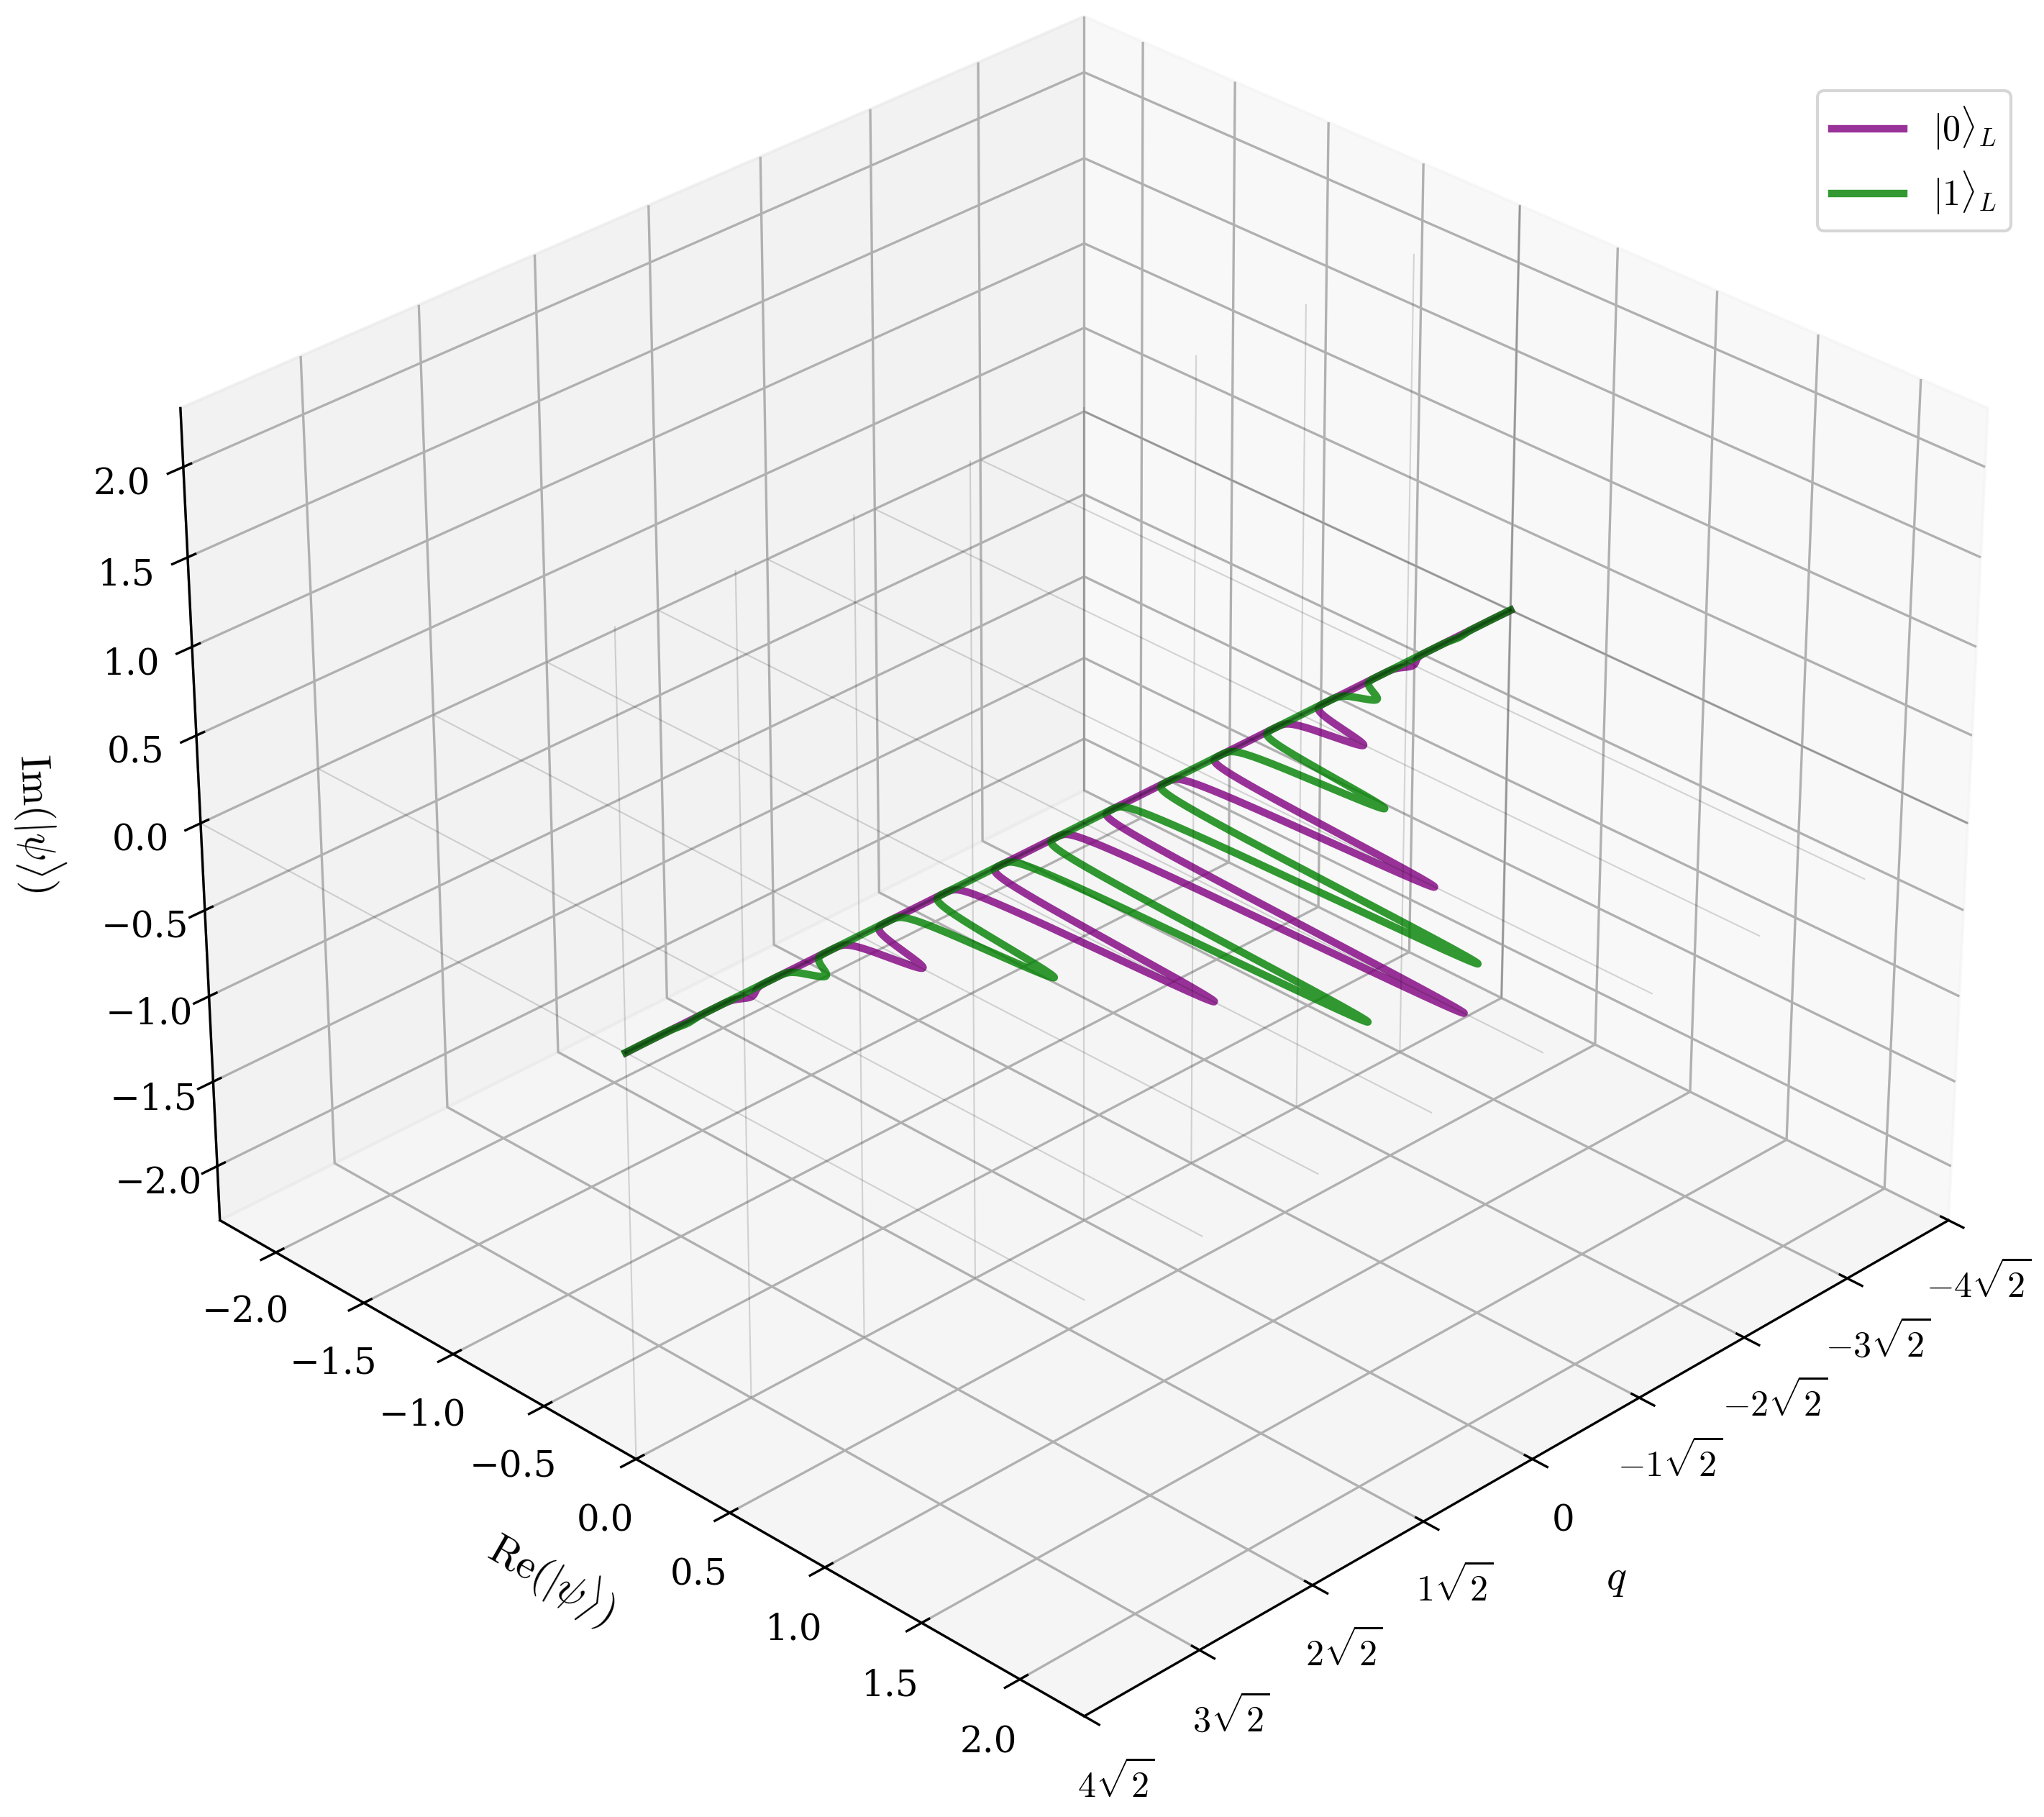
\includegraphics[valign=c, width=0.8\linewidth]{figures/qumodes/prelims/quantum_info/gkp_wavefunction_both}
    \end{equation}
    The logical operators are displacements by vectors in the dual lattice $\Lambda_\SSS^\perp$.
    We can choose as logical operators:
    \begin{equation}
        \hat{X}_L \coloneqq \hat{X}\left(\frac{1}{\sqrt{2}}\right)
        \qqquad \text{and} \qqquad
        \hat{Z}_L \coloneqq \hat{Z}\left(\frac{1}{\sqrt{2}}\right)
    \end{equation}
    These satisfy the required commutation relation $\hat{X}_L \hat{Z}_L = e^{i\pi} \hat{Z}_L \hat{X}_L = -\hat{Z}_L \hat{X}_L$ for Pauli operators.
    The algebraic distance of the code is $1/\sqrt{2}$, the length of the shortest non-trivial logical operator.
    The computational basis codestates are:
    \begin{equation}\label{eq:single_mode_square_GKP_computational_codestates}
        \ket{0}_L = \sum_{k \in \ZZ} \delta_{\sqrt{2}k}
        \qqquad \text{and} \qqquad
        \ket{1}_L = \sum_{k \in \ZZ} \delta_{1/\sqrt{2} + \sqrt{2}k}
    \end{equation}
    We can verify that $\hat{X}_L$ swaps these two states by shifting the comb by $1/\sqrt{2}$, and that $\ket{0}_L$ and $\ket{1}_L(x)$ are respectively the $+1$ and $-1$ eigenstates of $\hat{Z}_L$.
    In the Wigner function representation, these Dirac combs in position space become Dirac combs in phase space (though I guess a 2D comb isn't much of a comb anymore -- more of a hairbrush).
    Again, we haven't set up enough maths to prove it rigorously, but the logical $\ket{0}_L$ state has Wigner function:
    \begin{equation}
        W_{\ket{0}_L} = \sum_{j,k \in \ZZ} (-1)^{jk} \delta_{(\frac{1}{2\sqrt{2}}2j, \frac{1}{2\sqrt{2}}k)}
    \end{equation}
    The logical $\ket{1}_L$ state is obtained by applying $\hat{X}_L = \hat{X}(1/\sqrt{2})$ to $\ket{0}_L$, which translates the Wigner function by $(1/\sqrt{2}, 0)$ in phase space:
    \begin{equation}
        W_{\ket{1}_L} = \sum_{j,k \in \ZZ} (-1)^{(j+1)k} \delta_{(\frac{1}{2\sqrt{2}}2j, \frac{1}{2\sqrt{2}}k)}
    \end{equation}
    The phase space picture makes clear why this code can correct displacement errors: small displacement errors move the Wigner function slightly, but as long as the displacement is less than half the lattice spacing, we can identify which codestate we're closest to and apply a correction.
    Below we plot approximations of $W_{\ket{0}_L}$ and $W_{\ket{1}_L}$ respectively; that is, we view $\ket{0}_L$ and $\ket{1}_L$ as the functions in~\eqref{eq:dirac_comb_as_real_function}, and plot their Wigner transforms.
    We also project these Wigner functions onto the lattice on the floor; this is ultimately the easier way to visualise these functions!
    \begin{equation*}
        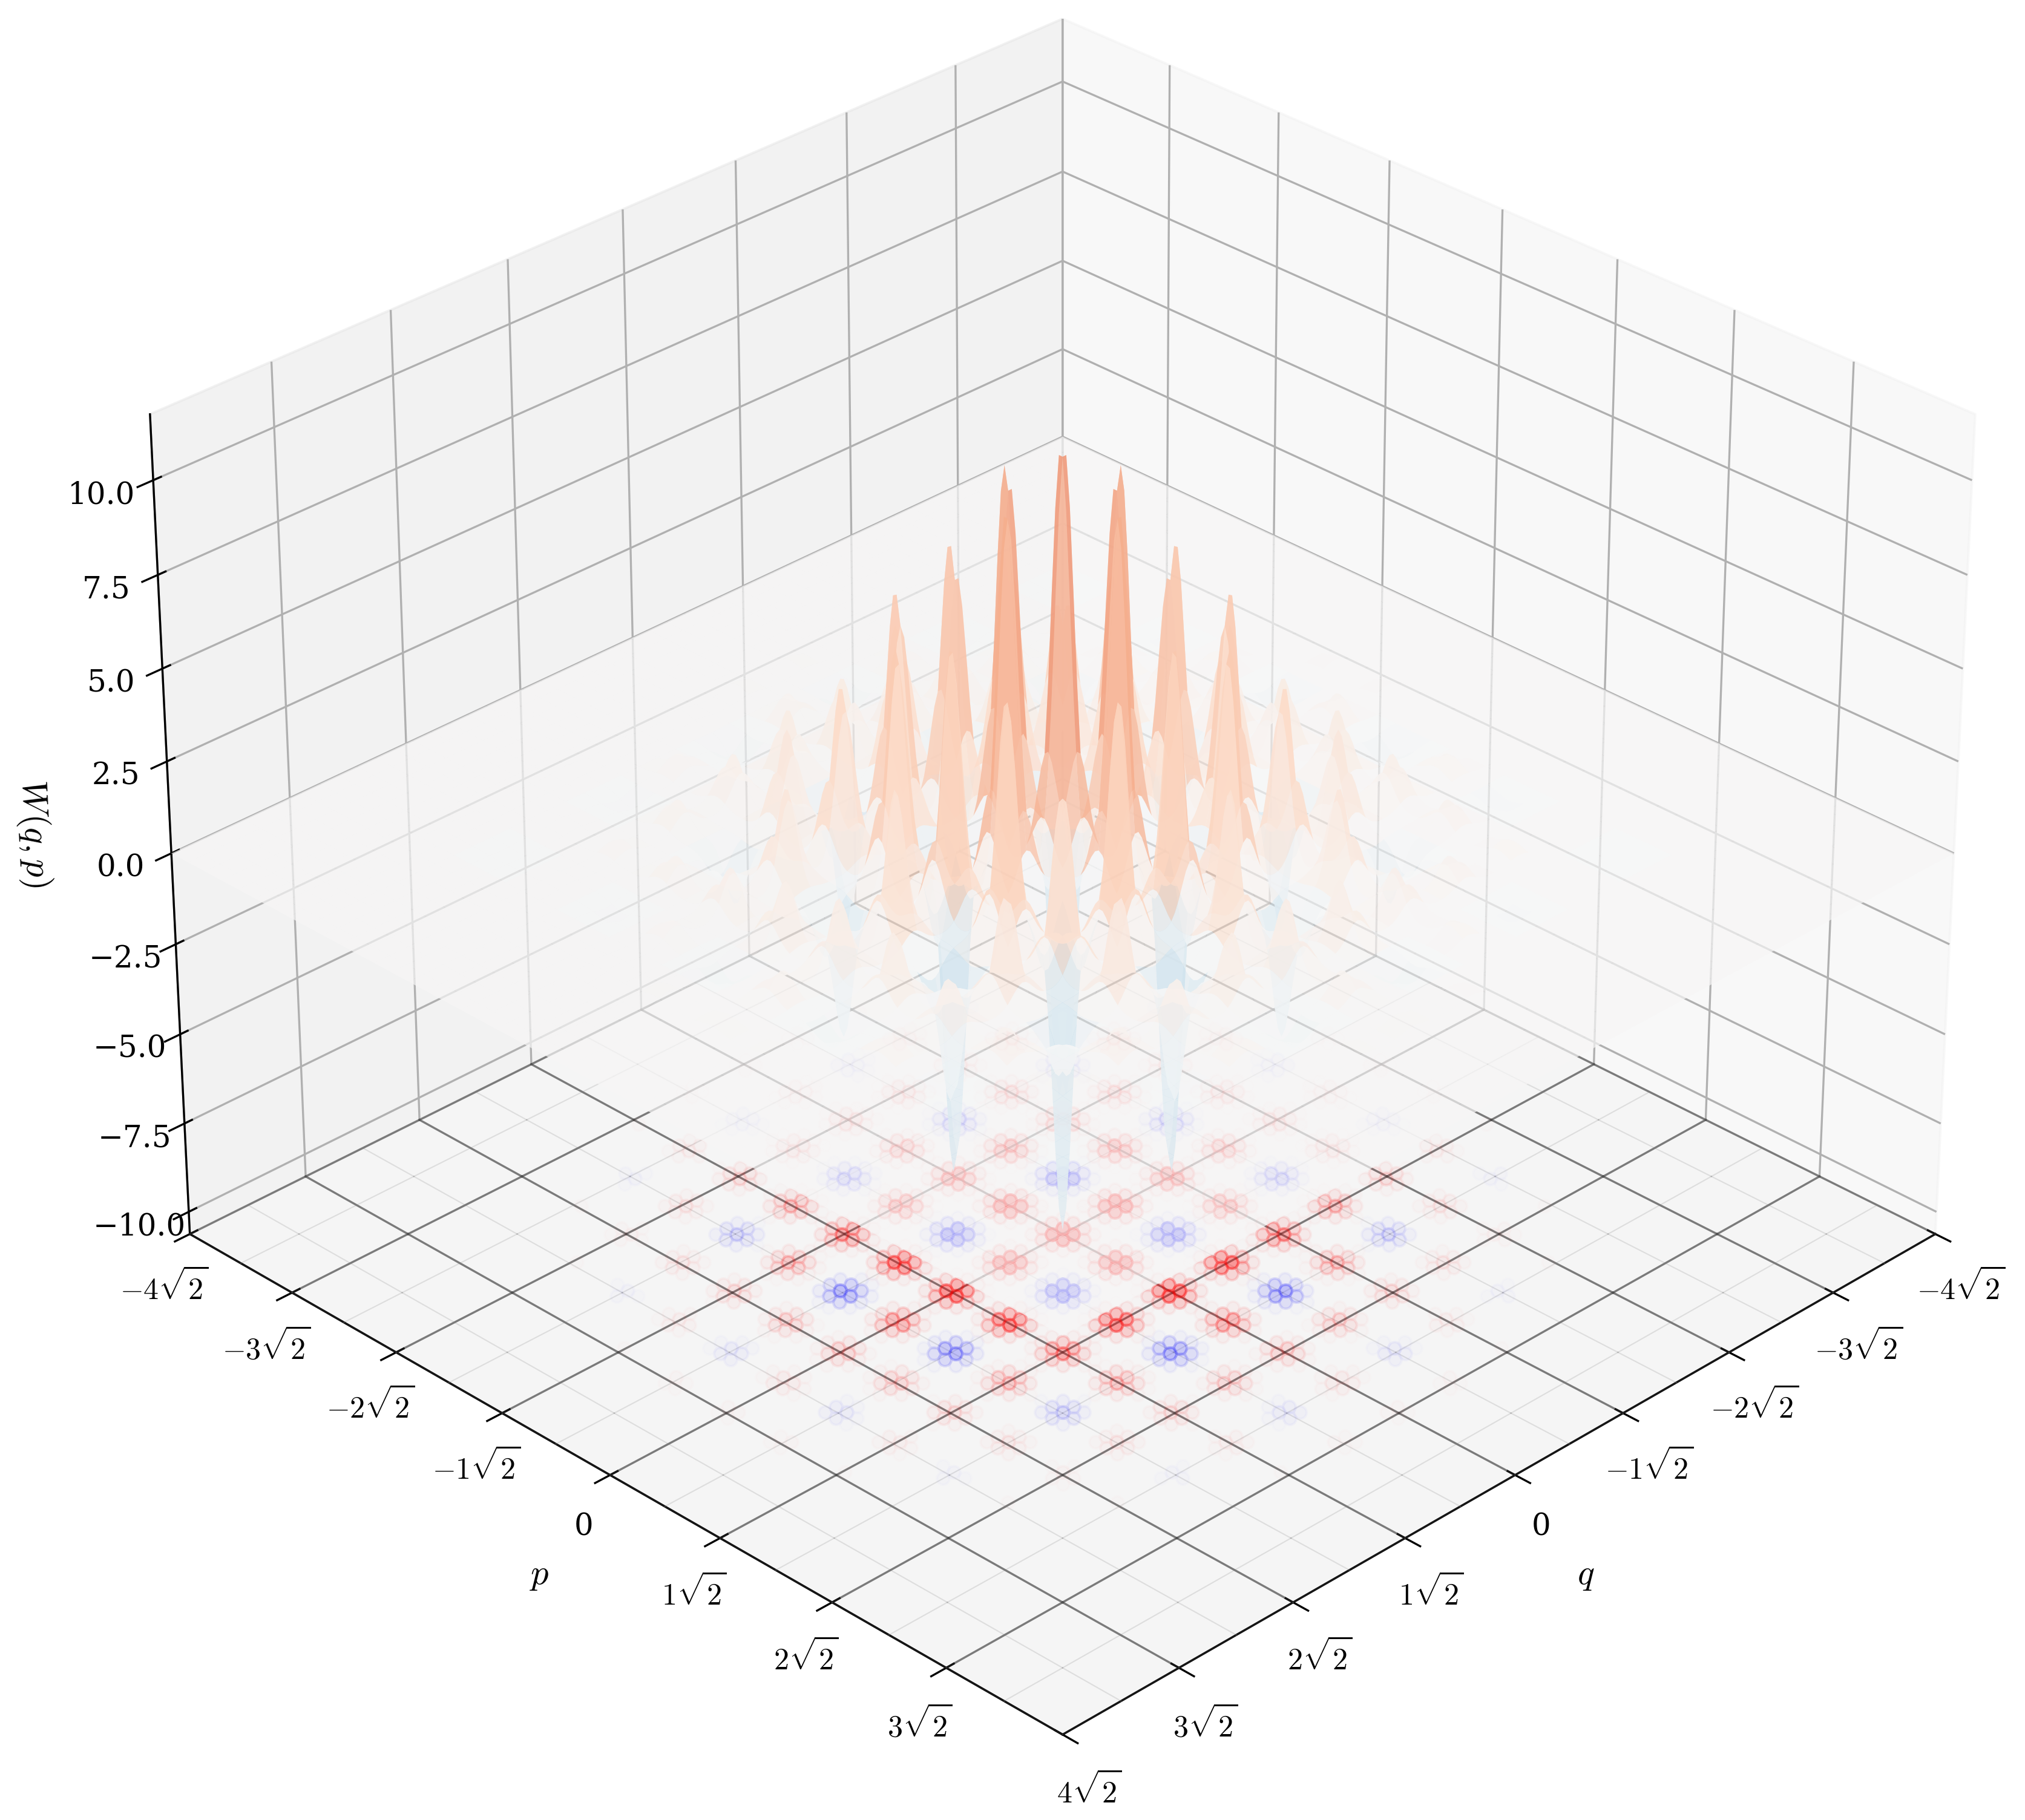
\includegraphics[valign=c, width=0.5\linewidth]{figures/qumodes/prelims/quantum_info/gkp_wigner_0_lattice}
        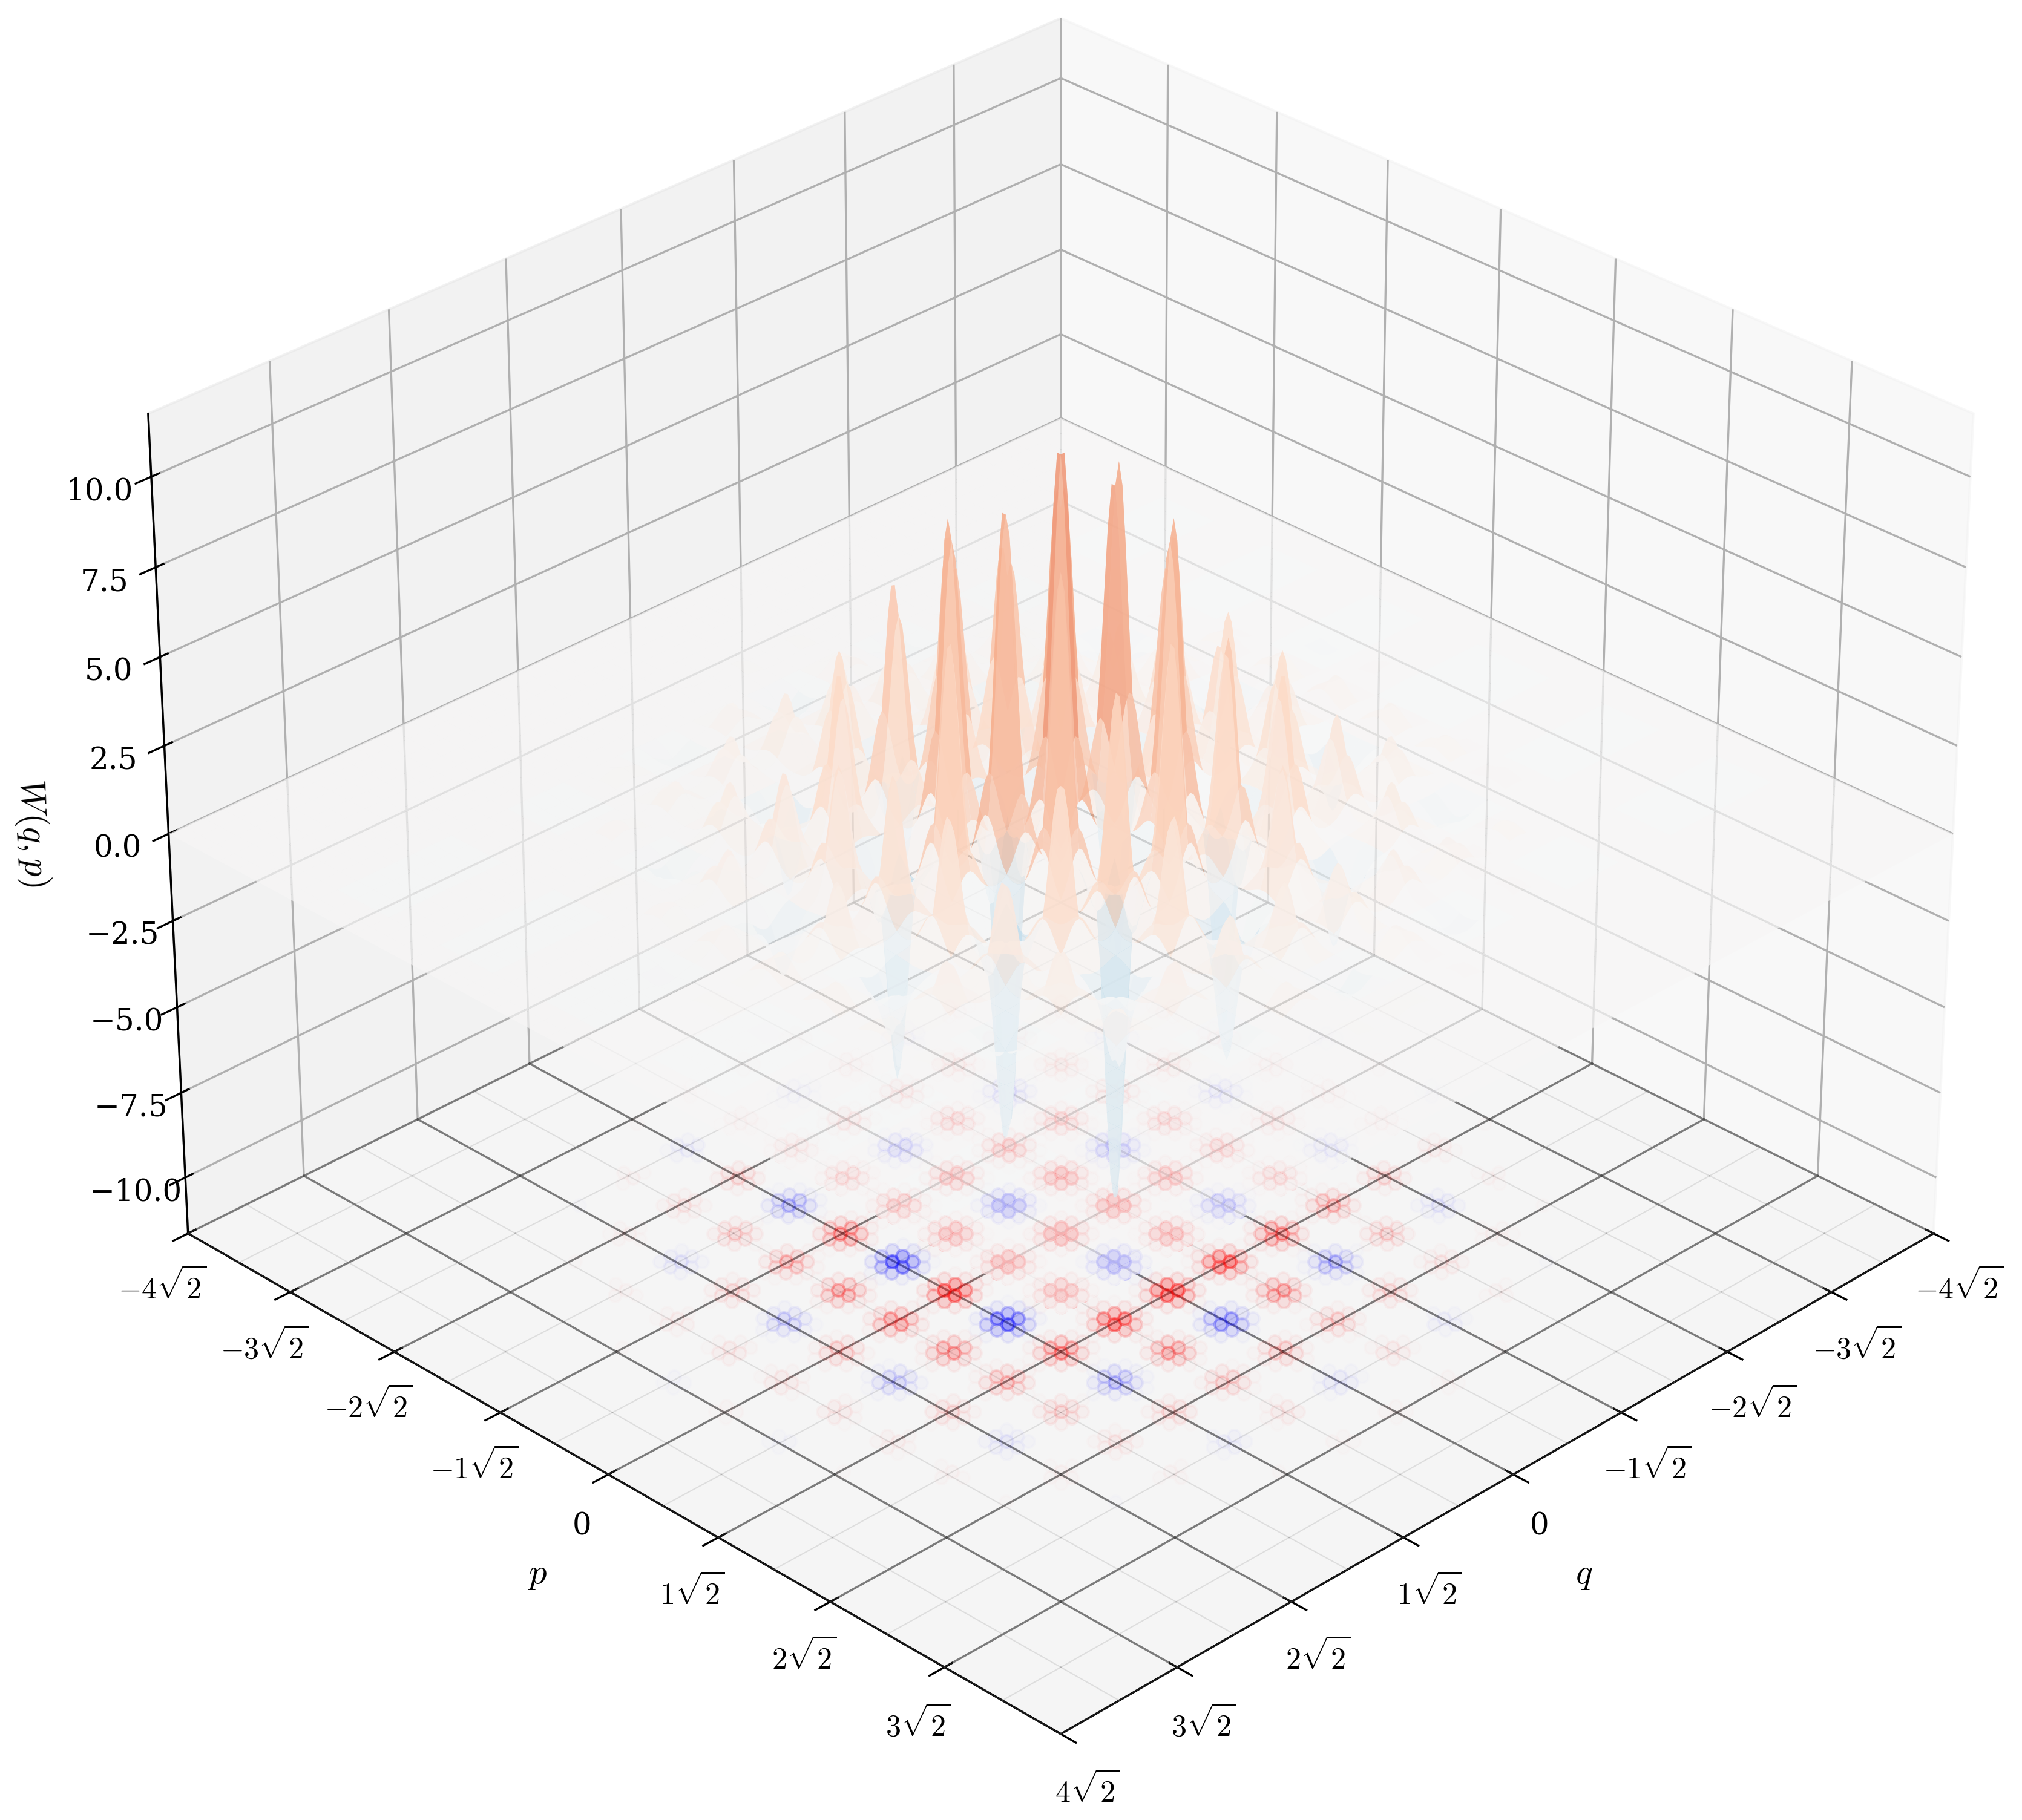
\includegraphics[valign=c, width=0.5\linewidth]{figures/qumodes/prelims/quantum_info/gkp_wigner_1_lattice}
    \end{equation*}
\end{example}

\begin{example}[Hexagonal lattice single-mode GKP]\label{ex:hexagonal_gkp}
    While the square lattice GKP code is arguably the simplest single-mode GKP code, the hexagonal lattice GKP code has a larger algebraic distance for the same lattice density.
    One choice of generator matrix for the self-dual hexagonal lattice is:
    \begin{equation}
        M_0 = \begin{pmatrix} 2 & 1 \\ 0 & \sqrt{3} \end{pmatrix}
    \end{equation}
    Scaling this by $\sqrt{d}$ to get $M = \sqrt{d}M_0$ again encodes a qudit into this qumode.
    The code's stabilizer group is then:
    \begin{equation}
        \SSS = \pres{\hat{D}(\sqrt{d}\tbinom{2}{\sqrt{0}}), \hat{D}(\sqrt{d}\tbinom{1}{\sqrt{3}})}
    \end{equation}
    The dual lattice $\Lambda_\SSS^\perp$ has generator $\frac{1}{\sqrt{d}}M_0$.
\end{example}

\begin{example}[Square lattice multi-mode GKP]\label{ex:square_multimode_gkp}
    GKP codes naturally extend to multiple qumodes.
    The self-dual hypercube lattice $\mathbb{Z}^{2n}$ has generator $I_{2n}$, which can be scaled by $\sqrt{d}$ to encode $n$ qudits into $n$ qumodes.
    The stabilizer group is:
    \begin{equation}
        \SSS = \pres{\hat{X}_j(\sqrt{2}), \hat{Z}_j(\sqrt{2}) : j = 1, \ldots, n}
    \end{equation}
    where $\hat{X}_j$ and $\hat{Z}_j$ act as displacements on the $j$th qumode only.
\end{example}

\begin{example}[$E_8$ lattice multi-mode GKP]\label{ex:E8_gkp}
    The most exotic GKP code we'll mention is defined via the self-dual $E_8$ lattice.
    A generating matrix for this is:
    \begin{equation}\label{eq:E8_lattice_generator_OG}
        M_0 =
        \begin{pmatrix}
            1 & 0 & 0 & 0 & 0 & 0 & 0 & 1/2 \\
            -1 & 1 & 0 & 0 & 0 & 0 & 0 & 1/2 \\
            0 & -1 & 1 & 0 & 0 & 0 & 0 & 1/2 \\
            0 & 0 & -1 & 1 & 0 & 0 & 0 & 1/2 \\
            0 & 0 & 0 & -1 & 1 & 0 & 0 & 1/2 \\
            0 & 0 & 0 & 0 & -1 & 1 & 0 & 1/2 \\
            0 & 0 & 0 & 0 & 0 & -1 & 1 & 1/2 \\
            0 & 0 & 0 & 0 & 0 & 0 & -1 & 1/2
        \end{pmatrix}
    \end{equation}
    As with all the other examples, we can scale this by $\sqrt{d}$ and define the stabilizer group accordingly.
    This then encodes four qudits into four qumodes.
    We will come back to this example right at the end of the thesis.
\end{example}

With specific examples out the way, we go back to the general definition to take a closer look at the codespace projector.
First, written out in full, the (infinite) GKP stabilizer group is:
\begin{equation}
    \mathcal{S} = \left\{ \prod_{j=1}^{2m} \hat{D}(\tbinom{\bsym{q}_j}{\bsym{p}_j})^{a_j} \ | \ \bsym{a} \in \mathbb{Z}^{2m} \right\}
\end{equation}
In discussing the codespace projector, it's useful to compare the GKP case to the qubit case.
So consider also a qubit stabilizer code defined by
\begin{equation}
    \SSS' = \pres{S_1, \ldots, S_r} \leq \PPP_n
\end{equation}
This has codespace projector defined as $\Pi_{\SSS'} = \frac{1}{|\SSS'|}\sum_{S \in \SSS'} S$, which can be rewritten as a product of projectors:
\begin{equation}
    \Pi_{\SSS'} = \prod_{j = 1}^r \frac{1}{2}(I + S_j) = \prod_{j = 1}^r \Pi_{S_j}
\end{equation}
Each such projector $\Pi_{S_j} = \frac{1}{2}(I + S_j)$ happens to be the projector corresponding to the outcome $m=1$ in the projective measurement defined by $S_j$.
So we can just measure this generating set of stabilizers and this will project us into the codespace (more accurately, it'll project us into the codespace of $\pres{m_1 S_1, \ldots, m_r S_r}$, where $m_j$ are the outcomes of these measurements.)

Now, the GKP code's projector $\Pi_\SSS = \sum_{S \in \SSS} S$ is the same, minus the normalization (which is impossible, since $\SSS$ is infinite).
This can again be written as a product of projectors:
\begin{equation}\label{eq:GKP_codespace_projector}
    \Pi_{\SSS}
    = \sum_{S \in \SSS} S
    = \sum_{\bsym{a} \in \ZZ^{2m}} \prod_{j=1}^{2m} \hat{D}(\tbinom{\bsym{q}_j}{\bsym{p}_j})^{a_j}
    = \prod_{j=1}^{2m} \sum_{a_j \in \ZZ} \hat{D}(\tbinom{\bsym{q}_j}{\bsym{p}_j})^{a_j}
\end{equation}
The difference here is that $\Pi_j \coloneqq \sum_{a_j \in \ZZ} \hat{D}(\tbinom{\bsym{q}_j}{\bsym{p}_j})^{a_j}$ is not one of the projectors making up the projective measurement defined by the normal operator $\hat{D}(\tbinom{\bsym{q}_j}{\bsym{p}_j}) = e^{-i2\pi \hat{\bsym{r}}(\tbinom{\boldsymbol{v}}{\boldsymbol{u}})}$.
So unlike in the qubit case, we can't just say that we're measuring a generating set of stabilizers and having that project us into the codespace (up to sector).
However, $\Pi_j$ is a projector in the projective measurement defined by the quadrature operator $\hat{\bsym{r}}(\tbinom{\bsym{q}_j}{\bsym{p}_j}) \bmod 1$.
So in the GKP setting, when we say we're measuring a stabilizer generator, this isn't literally true like it was in the qubit setting, but rather what we really mean is we're performing a homodyne measurement mod 1.

GKP codes are implemented exactly as qubit stabilizer codes are implemented: we repeatedly measure the set of stabilizer generators, and each consecutive pair of measurements will form a detector, which we use to detect and correct errors.







